
\section{Frequenzmessung I}
\label{section:frequenzmessung_1}
\begin{frame}%STARTCONTENT

\begin{columns}
    \begin{column}{0.48\textwidth}
    \begin{itemize}
  \item Abgleich von Funkgeräten
  \item Nach Reparatur oder durch Veränderungen durch Alterung
  \item \emph{Frequenzzähler} zur Messung von Oszillatorfrequenzen
  \end{itemize}

    \end{column}
   \begin{column}{0.48\textwidth}
       
\begin{figure}
    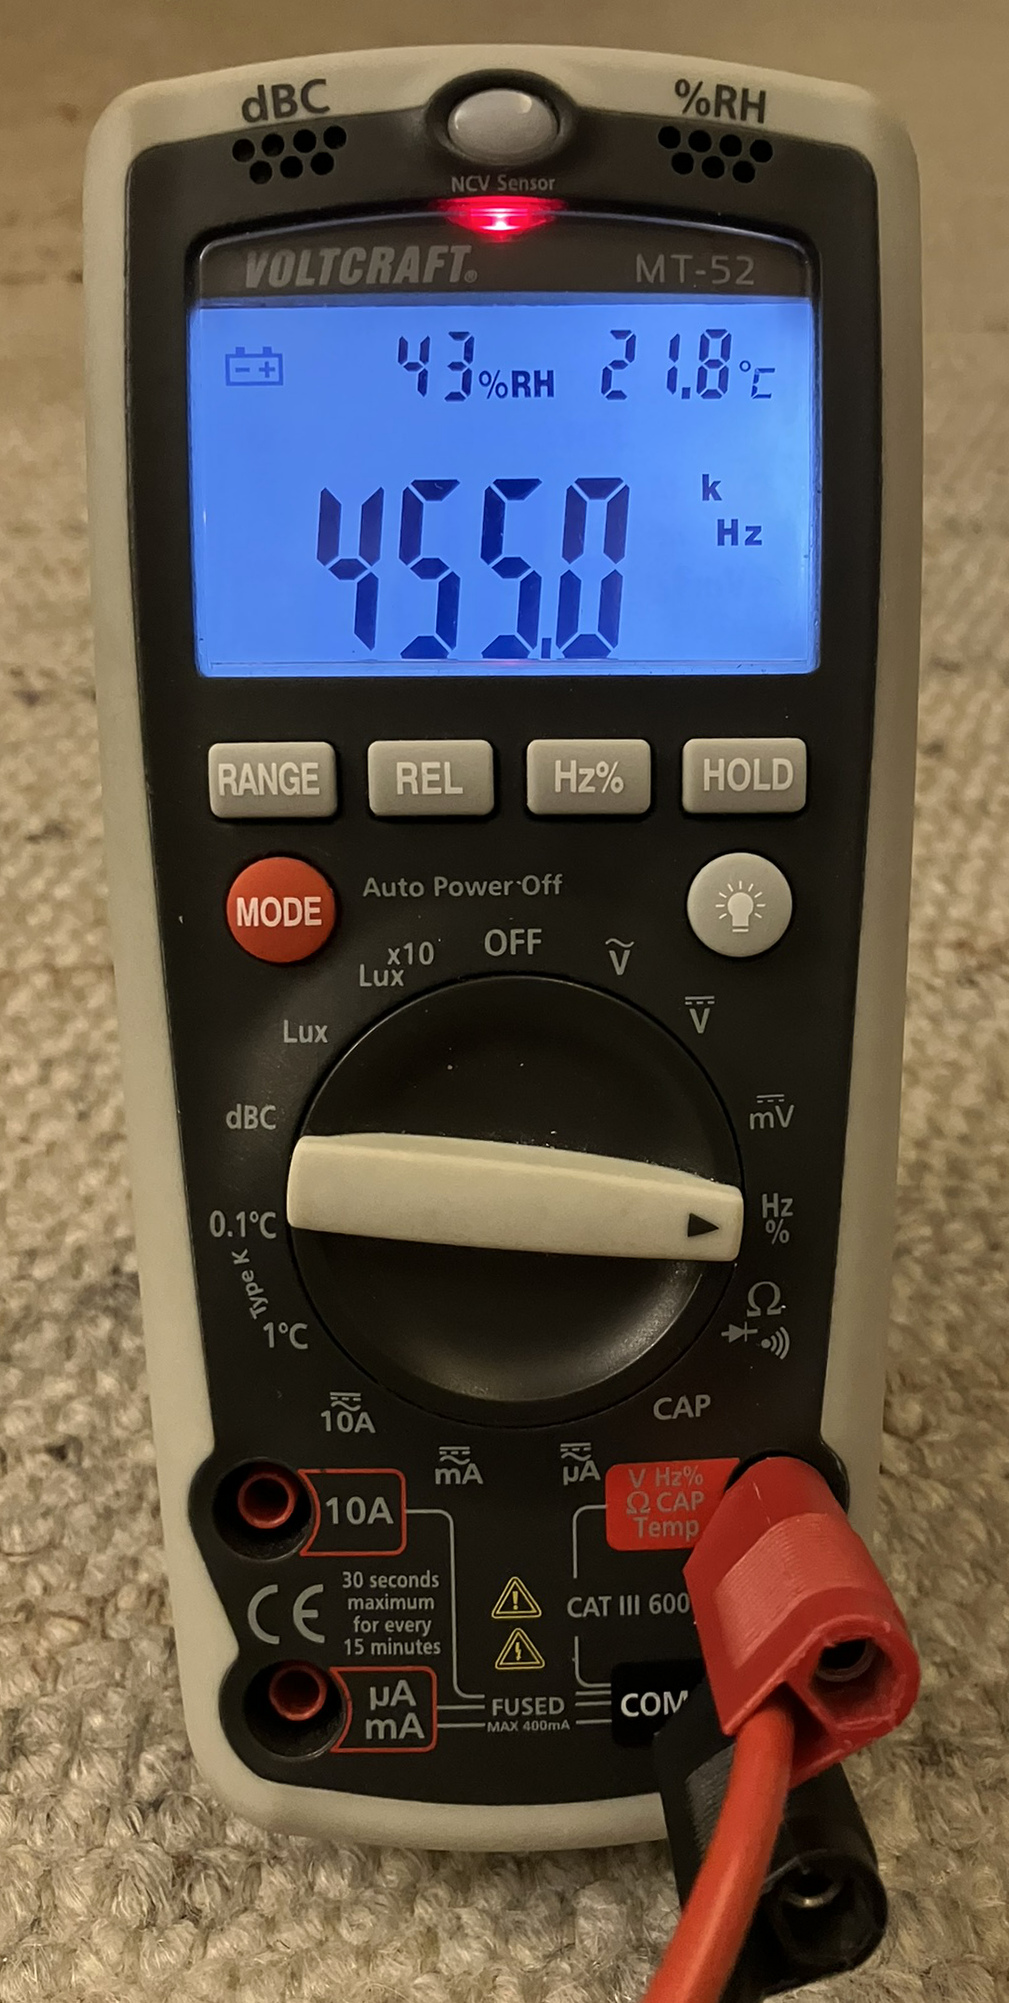
\includegraphics[width=0.85\textwidth]{foto/189}
    \caption{\scriptsize Multimeter, das im Frequenzmessbereich \qty{455}{\kilo\hertz} anzeigt. Darüber erscheinen ein Symbol für niedrige Batteriespannung, die Luftfeuchtigkeit und die Temperatur. Diese Werte haben nichts mit der Frequenzmessung zu tun.}
    \label{e_frequenzzaehler2}
\end{figure}

   \end{column}
\end{columns}

\end{frame}

\begin{frame}
\only<1>{
\begin{QQuestion}{EI501}{Womit kann die Frequenz eines unmodulierten Hochfrequenzsignals gemessen werden? Mit einem~...}{Frequenzzähler.}
{Widerstandsmessgerät.}
{Wechselspannungsmessgerät.}
{Wechselstromzähler.}
\end{QQuestion}

}
\only<2>{
\begin{QQuestion}{EI501}{Womit kann die Frequenz eines unmodulierten Hochfrequenzsignals gemessen werden? Mit einem~...}{\textbf{\textcolor{DARCgreen}{Frequenzzähler.}}}
{Widerstandsmessgerät.}
{Wechselspannungsmessgerät.}
{Wechselstromzähler.}
\end{QQuestion}

}
\end{frame}

\begin{frame}
\begin{columns}
    \begin{column}{0.48\textwidth}
    \begin{itemize}
  \item Anzeige der Frequenz
  \item Bei älteren Geräten steht hinten ein 10<sup>x</sup>-Multiplikator
  \end{itemize}

    \end{column}
   \begin{column}{0.48\textwidth}
       
\begin{figure}
    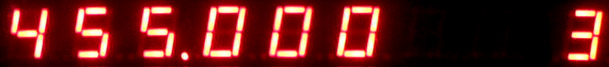
\includegraphics[width=0.85\textwidth]{foto/187}
    \caption{\scriptsize Display eines Frequenzzählers, der 455 · 10<sup>3</sup> Hz anzeigt}
    \label{e_frequenzzaehler1}
\end{figure}

   \end{column}
\end{columns}

\end{frame}

\begin{frame}
\begin{columns}
    \begin{column}{0.48\textwidth}
    \begin{itemize}
  \item Abgleichanleitung verlangt oft Einstellung bis auf eine bestimmte Abweichung
  \item z.B.  $\pm$ 10 Hz
  \item Stellenwert der Ziffern kennen
  \item Auf Komma und Einheitenpräfix oder Multiplikator achten
  \end{itemize}

    \end{column}
   \begin{column}{0.48\textwidth}
       
\begin{figure}
    \DARCimage{0.85\linewidth}{793include}
    \caption{\scriptsize Diese Anzeige stellt eine Frequenz in MHz dar. Das ist zugleich der Stellenwert der Ziffer vor dem Komma.}
    \label{e_frequenzzaehler_stellen}
\end{figure}


\begin{figure}
    \DARCimage{0.85\linewidth}{104include}
    \caption{\scriptsize Manche Anzeigen eines Frequenzzählers haben weniger Nachkommastellen}
    \label{e_frequenzzaehler_weniger_stellen}
\end{figure}


   \end{column}
\end{columns}

\end{frame}

\begin{frame}
\only<1>{
\begin{PQuestion}{EI502}{Das Bild stellt die Anzeige eines Frequenzzählers dar. Welchen Stellenwert hat die mit X gekennzeichnete Ziffer?}{ein Kilohertz}
{ein Hertz}
{hundert Hertz}
{zehn Hertz}
{\DARCimage{1.0\linewidth}{103include}}\end{PQuestion}

}
\only<2>{
\begin{PQuestion}{EI502}{Das Bild stellt die Anzeige eines Frequenzzählers dar. Welchen Stellenwert hat die mit X gekennzeichnete Ziffer?}{\textbf{\textcolor{DARCgreen}{ein Kilohertz}}}
{ein Hertz}
{hundert Hertz}
{zehn Hertz}
{\DARCimage{1.0\linewidth}{103include}}\end{PQuestion}

}
\end{frame}

\begin{frame}
\only<1>{
\begin{PQuestion}{EI503}{Das Bild stellt die Anzeige eines Frequenzzählers dar. Welchen Stellenwert hat die mit X gekennzeichnete Ziffer?}{ein Kilohertz}
{ein Hertz}
{hundert Hertz}
{zehn Hertz}
{\DARCimage{1.0\linewidth}{104include}}\end{PQuestion}

}
\only<2>{
\begin{PQuestion}{EI503}{Das Bild stellt die Anzeige eines Frequenzzählers dar. Welchen Stellenwert hat die mit X gekennzeichnete Ziffer?}{ein Kilohertz}
{ein Hertz}
{hundert Hertz}
{\textbf{\textcolor{DARCgreen}{zehn Hertz}}}
{\DARCimage{1.0\linewidth}{104include}}\end{PQuestion}

}
\end{frame}

\begin{frame}
\frametitle{Wertebereich}
\begin{itemize}
  \item Außerhalb des angegebenen Wertebereichs messen Frequenzzähler ungenau oder gar nicht
  \item Für höhere Frequenzen gibt es Frequenzteiler
  \item Angelegte Frequenz wird durch einen festen Wert geteilt
  \item Ergebnis wird als elektrische Schwingung ausgegeben
  \item \emph{Vorteiler} genannt, da zwischen Messobjekt und Zähler geschaltet
  \item 10:1-Teiler bei \qty{2,4}{\giga\hertz} $\rightarrow$ \qty{240}{\mega\hertz}
  \end{itemize}
\end{frame}

\begin{frame}
\only<1>{
\begin{QQuestion}{EI504}{Wenn ein 10:1-Frequenzteiler vor einem Frequenzzähler geschaltet wird und der Zähler \qty{14,5625}{\MHz} anzeigt, beträgt die tatsächliche Frequenz~...}{\qty{14,5625}{\kHz}.}
{\qty{1,45625}{\MHz}.}
{\qty{14,5625}{\MHz}.}
{\qty{145,625}{\MHz}.}
\end{QQuestion}

}
\only<2>{
\begin{QQuestion}{EI504}{Wenn ein 10:1-Frequenzteiler vor einem Frequenzzähler geschaltet wird und der Zähler \qty{14,5625}{\MHz} anzeigt, beträgt die tatsächliche Frequenz~...}{\qty{14,5625}{\kHz}.}
{\qty{1,45625}{\MHz}.}
{\qty{14,5625}{\MHz}.}
{\textbf{\textcolor{DARCgreen}{\qty{145,625}{\MHz}.}}}
\end{QQuestion}

}
\end{frame}%ENDCONTENT
